\section{Introduction to quantum optics}\index{Quantum optics}

\famousquote{All the fifty years of conscious brooding have brought me no closer to answer the question, `What are light quanta?'. Of course today every rascal thinks he knows the answer, but he is deluding himself.}{Albert Einstein}
\\

\dropcap{M}{uch} as the classical internet is heavily dependent upon optics to mediate communication, any future quantum internet will almost inevitably rely heavily on quantum optics to mediate quantum communication. It is therefore worth introducing the language and basic set of tools employed in quantum optics.

%
% Discrete-variables
%

\subsection{Discrete-variables}\index{Discrete-variables}

Like most things in the quantum world, light is discretised into fundamental, indivisible particles called \textit{photons}\index{Photons} -- light quanta\index{Quanta}. The most basic optical quantum state comprising photons is the \textit{photon-number state}\index{Photon-number!State} or \textit{Fock state}. These states form a discrete basis, labelled by the integer number of photons in the state,
\begin{align}
\ket{n},\,n\in\mathbb{Z}^+.	
\end{align}
The special case of $\ket{0}$ is referred to as the \textit{vacuum state}\index{Vacuum state}, since it contains no photons.

The Fock states can be thought of as the energy levels in a quantum harmonic oscillator\index{Harmonic oscillators}, and the energy\index{Photons!Energy} of the $n$-photon Fock state is therefore given by,
\begin{align}
E_n = \left(n+\frac{1}{2}\right)\hbar\omega,
\end{align}
where $\omega$ is the optical frequency\index{Optical!Frequency} (in radians per second).

A measurement in the photon-number basis is represented using a photon-number projector\index{Photon-number!Projector},
\begin{align}
\hat\Pi_n &= \ket{n}\bra{n},\nonumber\\
\sum_{n=0}^\infty \hat\Pi_n &= \hat\openone.
\end{align}

Any optical state in a single mode can be represented in the photon-number basis, which generalises to the multi-mode case in the obvious way. Such a representation is typically referred to as a \textit{discrete-variable} (DV) \index{Discrete-variables} representation, since photon-number is discretised.

In many cases it's convenient to represent states using photonic \textit{creation} ($\hat{a}^\dag$) and \textit{annihilation} ($\hat{a}$) operators\index{Creation operators}\index{Annihilation operators}. These (non-commuting) operators have the effect of acting upon a photon-number state and incrementing or decrementing the state's photon-number. Note that these operators are not unitary, and therefore do not represent legitimate quantum evolutions on their own. However, they may be used to construct unitary operators representing evolution processes. These operators satisfy the following basic algebraic properties:
\begin{align}
\hat{a}^\dag\ket{n} &= \sqrt{n+1}\ket{n+1},\nonumber\\
\hat{a}\ket{n} &= \sqrt{n}\ket{n-1},\nonumber\\
\hat{a}\ket{0} &= 0,\nonumber\\
\ket{n} &= \frac{1}{\sqrt{n!}}(\hat{a}^\dag)^n\ket{0},\nonumber\\
[\hat{a},\hat{a}^\dag] &= 1.
\end{align}

For multiple modes (1 and 2) the different creation operators commute, as do the respective annihilation operators,
\begin{align}
[\hat{a}^\dag_1,\hat{a}^\dag_2] &= 0,\nonumber\\
[\hat{a}_1,\hat{a}_2] &= 0.
\end{align}

A particularly useful and ubiquitous operator is the photon-number operator\index{Photon-number!Operator}, defined as,
\begin{align}
\hat{n}=\hat{a}^\dag\hat{a},
\end{align}
which satisfies the eigenvalue relation\index{Eigenvalue equation} with photon-number states,
\begin{align}
\hat{n}\ket{n} = n\ket{n}.	
\end{align}

%
% Continuous-variables
%

\subsection{Continuous-variables}\index{Continuous-variables}

A completely alternate, but entirely equivalent formalism for the representation of quantum optical states is in the \textit{continuous-variable} (CV) picture. Here we no longer think in terms of a discretised photon-number basis, but in terms of a continuous basis in the complex plane, referred to as \textit{phase-space}\index{Phase-space}, completely analogous to the familiar classical phase-space. This alternate representation is introduced purely as a matter of convenience, since some states (typically referred to as CV states), are particularly well-suited to elegant representation in this picture, as are some types of evolution.

In the CV picture, instead of representing states using photonic creation operators, we express them in terms of the \textit{position} ($\hat x$)\index{Position operator} and \textit{momentum} ($\hat p$)\index{Momentum operator} operators, which are related to the creation and annihilation operators as,
\begin{align}
\hat x &=    \sqrt{\frac{\hbar}{2 \omega}}(\hat a + \hat a^\dag), \nonumber \\
\hat p &= -i \sqrt{\frac{\hbar  \omega}{2}}(\hat a - \hat a^\dag), 
\end{align}
where $\omega$ is the optical frequency\index{Optical!Frequency}. These operators obey the commutation relation,
\begin{align}
[\hat x, \hat p] = i \hbar.
\end{align}

The position and momentum operators represent the \textit{quadratures}\index{Quadratures} of a mode, and correspond to the real and imaginary components of a harmonic oscillator's\index{Harmonic oscillator} amplitude.

The \textit{position representation} of an optical state corresponds to expressing a state vector $\ket{\psi}$ in the position basis\index{Position basis representation},
\begin{align}
\ket{\psi} = \int \psi(x)\ket{x}\, dx,
\end{align}
where $\ket{x}$ are the eigenstates of the position operator,
\begin{align}
	\hat{x}\ket{x}=x\ket{x}.
\end{align}
Here the wave-function in the position representation\index{Position basis representation} is defined as,
\begin{align}
\psi(x) = \braket{x|\psi}.
\end{align}
The state can similarly be expressed via a \textit{momentum representation}\index{Momentum basis representation},
\begin{align}
	\ket\psi = \int {\tilde\psi}(p) \ket{p}\, dp,
\end{align}
where,
\begin{align}
	{\tilde\psi}(p) &= \braket{p|\psi},\nonumber\\
	\hat{p}\ket{p} &= p\ket{p}.
\end{align}

The quadrature eigenstates\index{Quadratures!Eigenstates} are mutually related to each other by a Fourier transform\index{Fourier transform},
\begin{align}
\ket{x} &= \frac{1}{\sqrt{\pi}} \int_{-\infty} ^\infty e^{-2 i x p} \ket{p} \,dp,\nonumber \\
\ket{p} &= \frac{1}{\sqrt{\pi}} \int_{-\infty} ^\infty e^{2 i x p} \ket{x} \,dx.
\end{align}

A particularly ubiquitous state that emerges in CV representations is the \textit{coherent state}\index{Coherent states}, which closely approximates classical laser light\index{Laser},
\begin{align}\index{Coherent states}
\ket{\alpha} &= e^{-\frac{|\alpha|^2}{2}} \sum_{n=0}^\infty \frac{\alpha^n}{\sqrt{n!}} \ket{n},\nonumber\\
\hat{a}\ket{\alpha} &= \alpha\ket{\alpha},
\end{align}
where \mbox{$\alpha\in\mathbb{C}$} is the complex coherent amplitude. Writing the coherent amplitude as,
\begin{align}
	\alpha=re^{i\theta},
\end{align}
$r$ can be interpreted as the strength of the classical field, and $\theta$ as its local phase.

Note that the coherent state has indeterminate photon-number (and hence energy) -- it is in fact a coherent superposition of \textit{all} photon-numbers (except when \mbox{$\alpha=0$}). However, the \textit{mean} photon-number\index{Coherent states!Mean photon-number} is a useful quantity, given by,
\begin{align}
\bar{n} = |\alpha|^2.
\end{align}

The phase-space representation for a coherent state is a circular `blob'\index{Blob} with mean $\alpha$ in the complex plane\index{Complex plane}, shown in Fig.~\ref{fig:phase_space}. The variance of the blob is indicative of the quantum uncertainty\index{Uncertainty} of the field in the two quadrature directions.

\begin{figure}[!htbp]
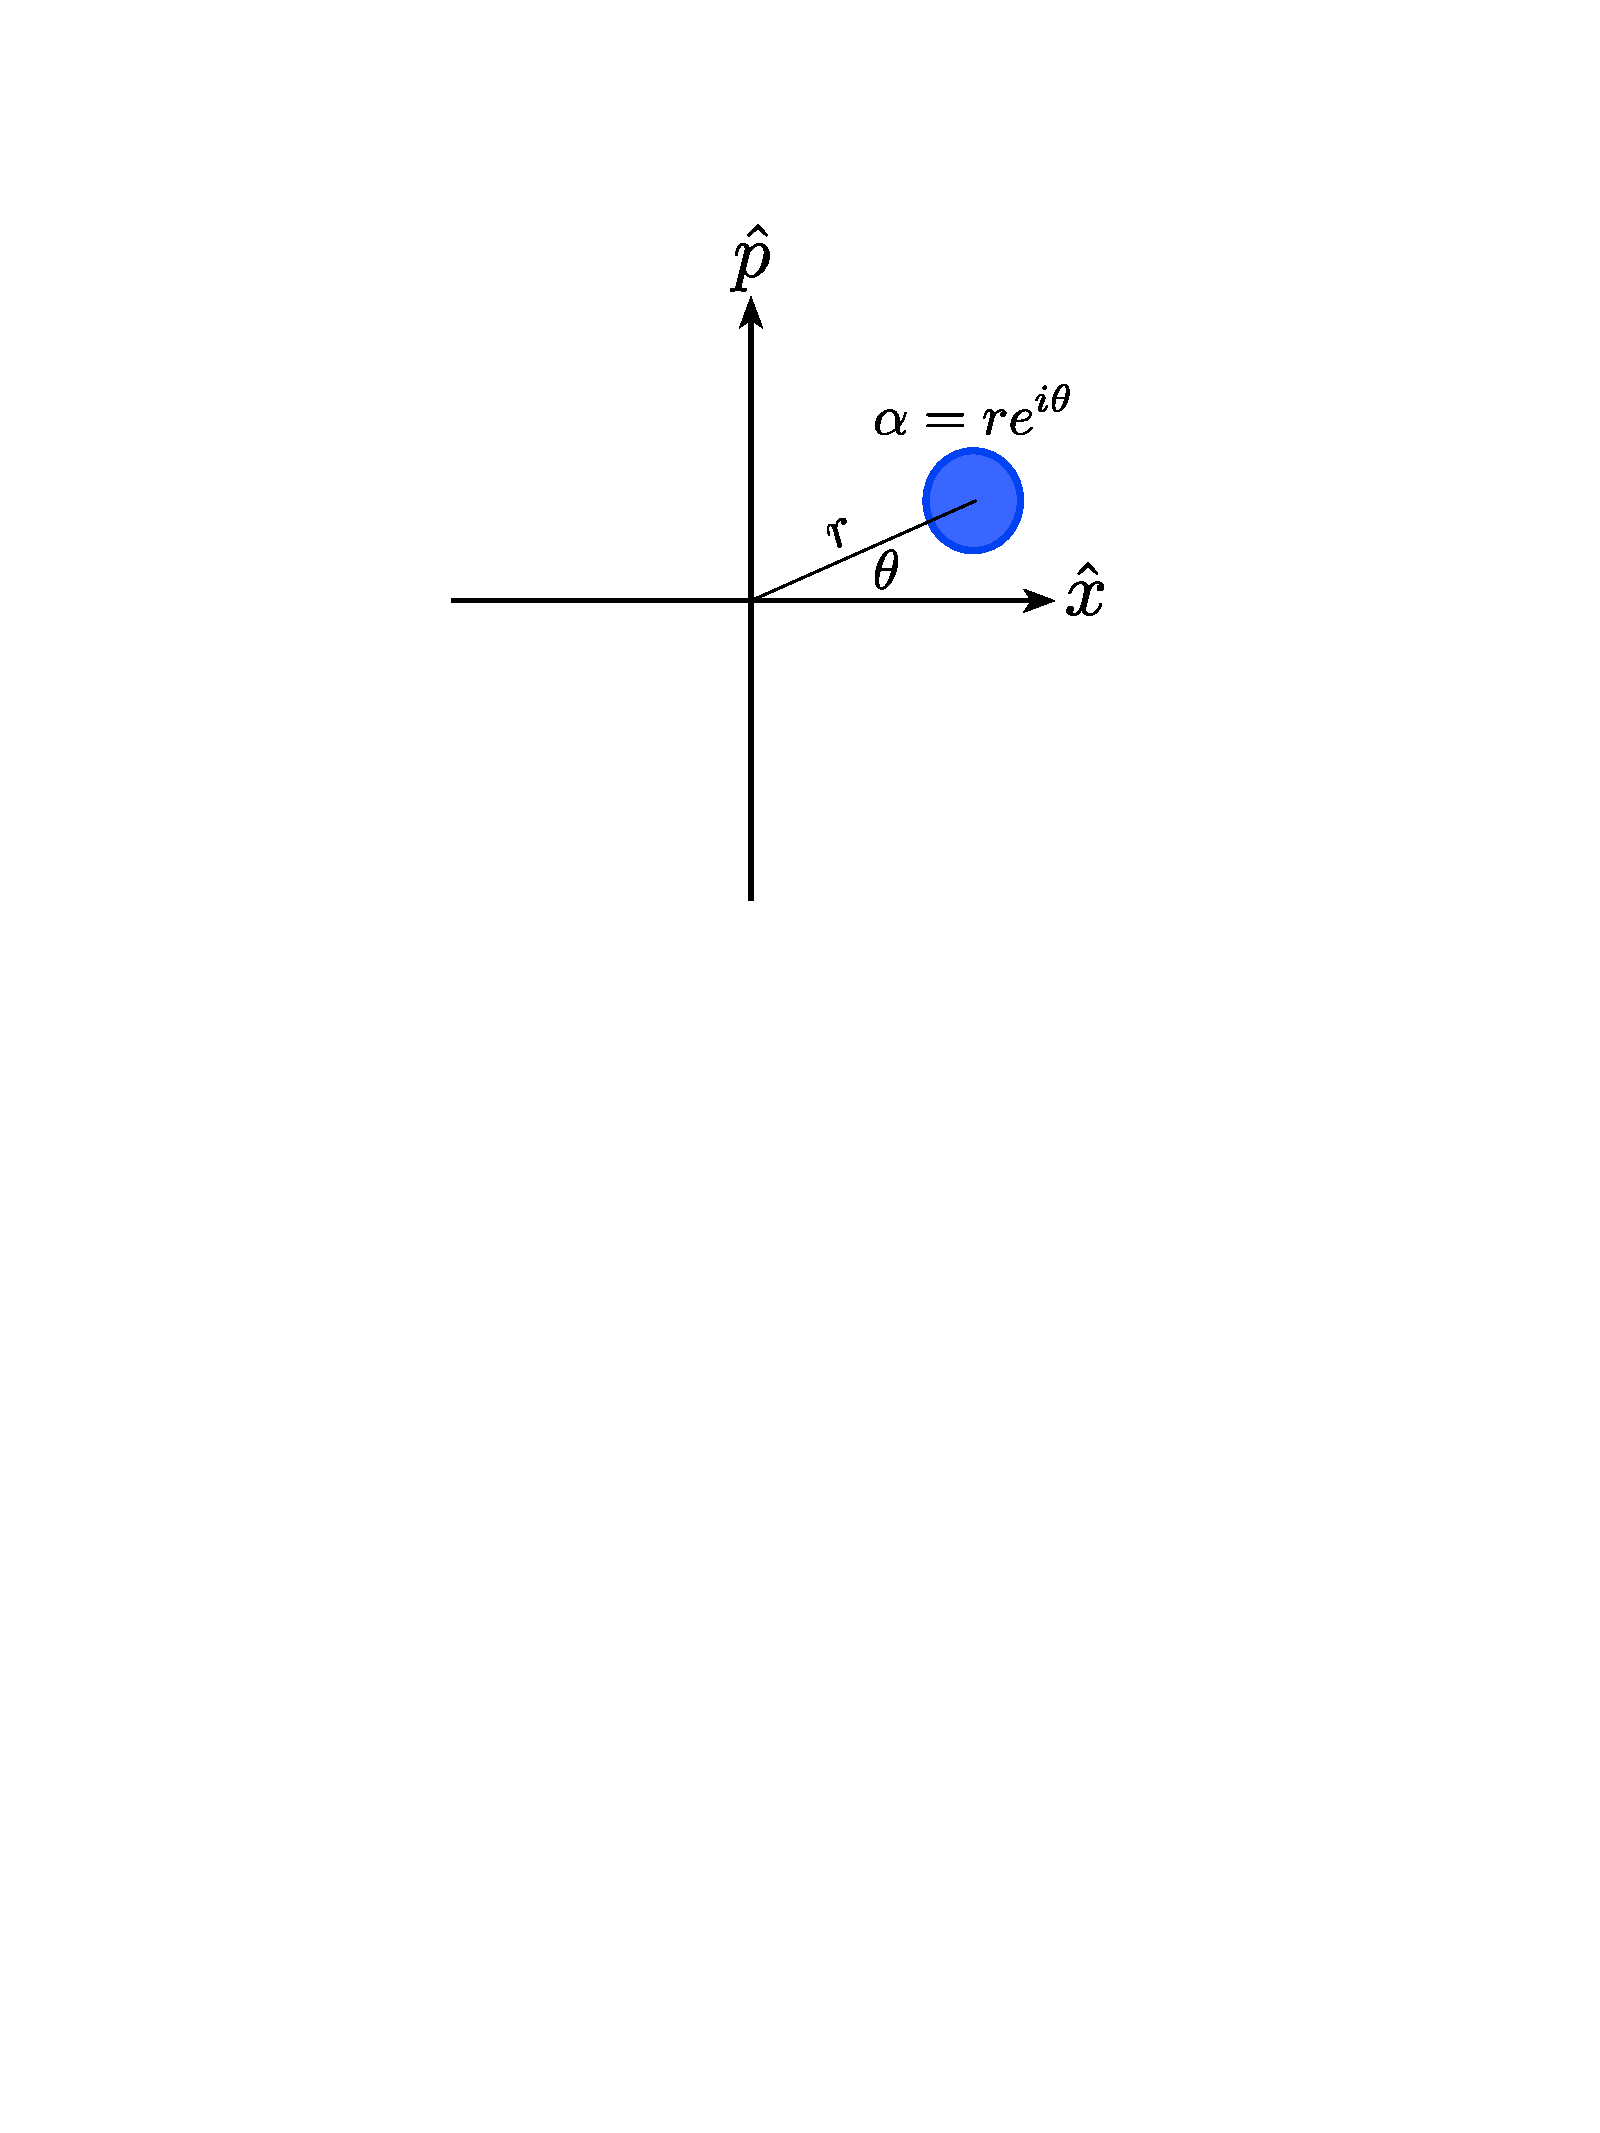
\includegraphics[clip=true, width=0.4\textwidth]{phase_space}
\captionspacefig \caption{Phase-space representation for a coherent state of complex amplitude \mbox{$\alpha=re^{i\theta}$}, where $r$ can be regarded as the field strength, and $\theta$ its phase.}\label{fig:phase_space}
\end{figure}